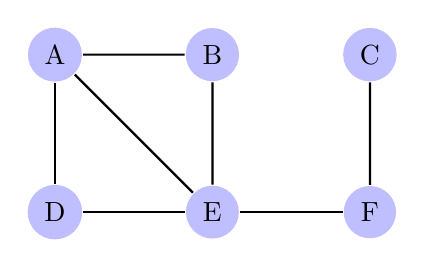
\begin{tikzpicture}
[thick,scale=.8,auto=left,node distance=2cm,every node/.style={circle,fill=blue!25}]
  \node (n6) {D};
  \node (n4) [above of=n6] {A};
  \node (n5) [right of=n6] {E};
  \node (n1) [right of=n4] {B};
  \node (n2) [right of=n5] {F};
  \node (n3) [right of=n1] {C};
  \foreach \from/\to in {n6/n4,n5/n1,n2/n5,n2/n3,n1/n4,n6/n5,n4/n5}
    \draw (\from) -- (\to);
\end{tikzpicture}
